AngularJS � un framework open-source per la creazione di \textit{single-page application}. Una applicazione single-page � una pagina web che carica dinamicamente dati dal server attraverso l'utilizzo di comunicazioni asincrone. 
Dal punto di vista dell'utente utilizzatore di questo tipo di applicazioni, la principale differenza con le comuni applicazioni web � la modalit� di navigazione. Muovendosi da una pagina all'altra, infatti, il client non richiede nuove pagine al server, bens\'{\i} esegue richieste in \textit{background} e carica dinamicamente i nuovi contenuti all'interno della pagina corrente con l'utilizzo di JavaScript. 

Il principale vantaggio offerto dalle applicazioni single-page si manifesta durante operazioni di gestione dei dati utente. Nelle comuni applicazioni web, infatti, i dati di sessione sono passati da una pagina alla successiva utilizzando svariate tecniche. Questa operazione � resa necessaria dalla natura \textit{state-less} del protocollo HTTP. Le single-page application risolvono alla radice il problema evitando il cambio di pagina e inviando i dati di autenticazione al server solo quando l'utente esegue operazioni per le quali � richiesta la sua identificazione.

L'utilizzo di AngularJS permette inoltre di realizzare applicazioni web utilizzando un pattern \textit{Model-View-ViewModel} (MVVM), semplificando molto la testabilit� del sistema. Una delle grandi problematiche di cui risentono le applicazioni web classiche infatti � la possibilit� di testare il codice che le compone. Tipicamente questa difficolt� nasce dal fatto che la logica applicativa e quella di visualizzazione sono codificate simultaneamente e quindi strettamente legate tra loro.

Il pattern MVVM facilita il processo di \textit{testing} delle applicazioni separando nettamente le competenze di ogni componente software che partecipa nel sistema. Questo pattern si basa sulla identificazione di tre componenti fondamentali:

\begin{description}
\item[Model] � la parte del sistema che si occupa di trattare i dati, tipicamente � implementata impiegando librerie per l'accesso a database oppure servizi esterni utilizzati come sorgenti di dati per l'applicazione.
\item[View] � l'interfaccia grafica vera e propria. Nel caso di applicazioni web si identifica spesso con le porzioni di codice HTML e quello CSS utilizzato per definire lo stile.
\item[ViewModel] implementa la logica applicativa, anche definita \textit{logica di business}. In questo strato software � possibile trovare algoritmi per la manipolazioni dei dati specifici dell'applicazione e funzionalit� per la gestione delle interazioni dei diversi servizi applicativi.
\end{description}

Le tre componenti del pattern MVVM cooperano tra loro scambiandosi messaggi secondo interfacce definite in fase di design dell'applicazione. La figura \ref{fig:mvvvm} mostra le principali interazioni richieste per permettere la completa collaborazione di tutte le componenti software.\\

\begin{figure}[h]
\centering
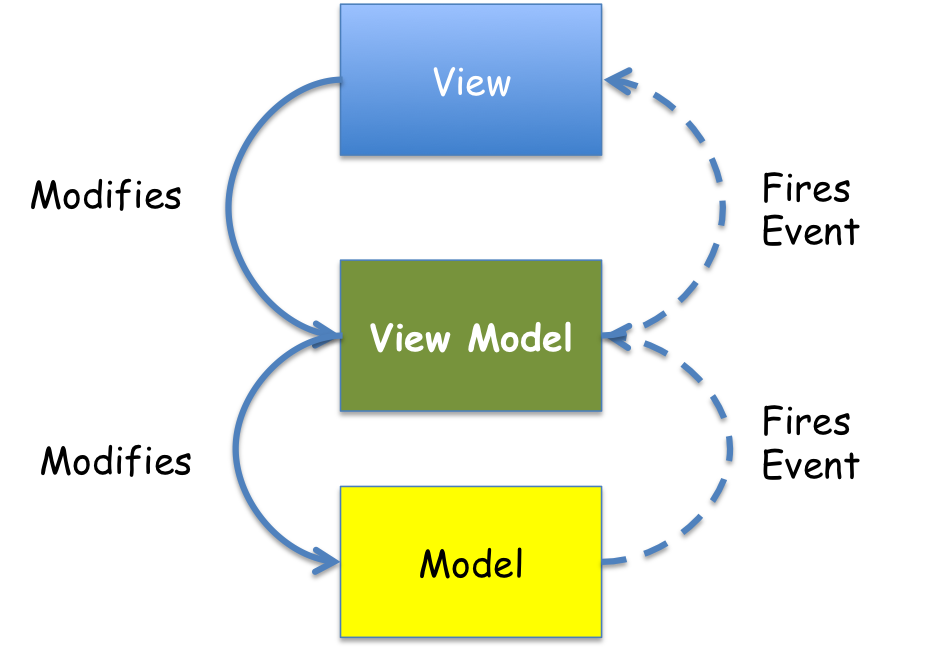
\includegraphics[width=0.7\linewidth]{./img/mvvm.png}
\caption[Schema delle comunicazioni nel modello MVVM]{Schema delle comunicazioni nel modello MVVM}
\label{fig:mvvvm}
\end{figure} 

Tipicamente questo approccio porta ad avere Model e ViewModel popolati con la maggior parte del codice applicativo, che, di conseguenza, viene rimosso dalla View. Il vantaggio dell'utilizzo dell'MVVM risiede proprio nel fatto che la sezione View, tipicamente complessa da testare, diventa molto semplice e di fatto � quasi inutile eseguire test sul codice che la genera.

La principale funzionalit� fornita da AngualrJS � il \textit{binding} dinamico delle variabili JavaScript con i controlli HTML presenti nella pagina. Il binding � una operazione che permette di collegare una parte di Model con una porzione definita di View. Tipicamente questa funzionalit� � utilizzata per collegare una variabile JavaScript con un controllo HTML, il binding garantisce che quando la variabile assume un nuovo valore, questo sia mostrato sulla interfaccia e, viceversa, quando un utente modifica il valore nella vista, questo venga immediatamente riflesso sulla variabile nel modello. Questo tipo di binding � definito \textit{bidirezionale} o \textit{two-way data binding}.

Il binding � una funzionalit� molto interessante, perch� solleva il programmatore dall'incombenza di mantenere la coerenza tra dati e interfaccia. Automatizzando questa operazione si ottiene anche una semplificazione del codice e una maggiore garanzia di funzionamento dell'applicazione. 

Per implementare il binding bidirezionale, AngularJS si serve di nuovi costrutti che arricchiscono il vocabolario a disposizione del programmatore per la stesura del codice HTML. Segue un esempio di codice contenente i costrutti AngularJS per realizzare un binding.

Contenuto del file \verb|view.html|:
\begin{verbatim}
<!doctype html>
<html ng-app='greetingsApp'>
  <head>
    <script src="angular.min.js"></script>
    <script src="app.js"></script>
  </head>
  <body ng-controller="GreetingsCtrl">
    Hello {{subject}}!
  </body>
</html>
\end{verbatim}

Contenuto del file \verb|app.js|:
\begin{verbatim}
angular.module('greetingsApp', [])
.controller('GreetingsCtrl', function ($scope) {
  $scope.subject = 'World';
});
\end{verbatim}

Esaminando il codice HTML del file view.html nell'esempio, si nota innanzitutto la necessit� di importare libreria JavaScript \verb|angular.min.js| nella pagina web. Questa operazione permette di utilizzare AngularJS all'interno della pagina stessa. Per attivare la libreria all'interno della pagina web �, inoltre, necessario specificare l'attributo \verb|ng-app|. All'applicazione nell'esempio � stato dato nome \verb|greetingsApp|.

AngularJS necessita di uno \textit{scope} nel quale monitorare le variabili che fanno uso del binding. Esso � definito con il l'attributo \verb|ng-controller|. Nell'esempio riportato lo scope sar� esteso a tutto il contenuto del tag \verb|body|. All'interno dello scope, si identificano le variabili della view agganciate al modello con l'utilizzo di una doppia parentesi graffa \verb|{{}}|.

Nell'esempio, la logica dell'applicazione risiede nel file \verb|app.js|, infatti al suo interno � possibile identificare una dichiarazione di controller e una funzione che ne implementa il comportamento. Nel caso riportato il comportamento � molto semplice, si limita all'assegnamento di una variabile utilizzata come modello. 

AngularJS fornisce un insieme piuttosto nutrito di librerie di utilit� che risolvono i pi� comuni problemi di comunicazione con sorgenti esterne di dati. Mole.io utilizza una di queste librerie per mettere in comunicazione i modelli AngularJS con una API REST presente sul server che si occupa di fornire i dati necessari a popolare le variabili. Non appena viene eseguito l'aggiornamento di tali variabili, AngularJS provvede ad aggiornare l'interfaccia utente con i dati ottenuti utilizzando codice molto simile a quello presente nell'esempio riportato precedentemente.

La struttura di questo framework, per sua natura, induce ad un design delle applicazioni per \textit{componenti} indipendenti ma comunicanti. E' possibile infatti immaginare una pagina web contenente diversi costrutti \verb|ng-controller|, ognuno dei quali si occupa di aggiornare una porzione della View con logiche specifiche. Non � difficile comprendere come questo approccio possa favorire la scrittura di software di buona qualit�, attraverso il riuso di componenti e lo studio attento della separazione delle responsabilit� di ogni componente. 

AngularJS utilizza il formato \textit{JavaScript Object Notation} (JSON) per lo scambio di dati tra il backend e i modelli. In \ref{crockford2008javascript} Douglas Crockford illustra questo formato da lui ideato. La definizione di JSON � aderente alle specifiche ECMA-262 del Dicembre 1999, e permette a JavaScript di interpretare questo formato nativamente. JSON quindi � un formato facilmente maneggiabile sia lato frontend, sia lato backend, questo ha contribuito a farlo diventare molto famoso e utilizzato per la realizzazione di applicazioni Node.js.

Per la realizzazione della parte fontend di Mole.io sono state utilizzate diverse librerie JavaScript e framework di supporto alla stesura del codice HTML. Di seguito saranno illustrate due importanti librerie  

-----------------

d3, bootstrap 

